\begin{pastexam}[label={px:ntu-109-ee-ds-22}]{臺大電機所 109 學年度（B）第 22 題}
（複選；每題 4 分，每答錯一個選項倒扣 0.8 分至該題 0 分止）

Consider the AA tree in Fig.3
\begin{enumerate}[label=(\Alph*)]
\item Key 4 and key 63 have the same level.
\item Key 62 and key 69 have the same level.
\item In Fig.3, after inserting the key 1, the key 4 is in the same level of key 42.
\item In Fig.3, after inserting the key 61, the parent of key 61 is key 62.
\item In Fig.3, after inserting the key 88, the parent of key 86 is key 77.
\end{enumerate}

\begin{center}
\begin{tikzpicture}[x=1.45cm,y=1.45cm,v/.style={draw,thick,circle,minimum size=5.6mm,inner sep=0pt,font=\scriptsize\sffamily},>={Stealth[length=1.8mm]}]
  \foreach \n/\x/\y in {77/7.40/9.51,42/6.02/10.21,63/6.73/10.21,90/8.68/10.21,4/5.03/11.03,15/5.68/11.03,62/6.46/11.03,69/7.19/11.03,79/7.79/11.03,86/8.43/11.03,93/9.15/11.03} {
    \node[v] (\n) at (\x,-\y) {\n};
  }
  \foreach \a/\b in {77/42,77/90,42/63,42/4,4/15,63/62,63/69,90/79,90/93,79/86} { \draw[->] (\a) -- (\b); }
\end{tikzpicture}\\ Fig.3 AA tree
\end{center}
\end{pastexam}

\begin{pastsoln}
答案：(B)、(E)。

AA 樹不在資結書的範圍，這裡先把規則講清楚。 AA 樹是紅黑樹的簡化版：每個節點存一個\textbf{層級}
（level），葉節點的層級是 $1$；
\begin{enumerate}
\item 左子節點的層級恰好比父節點小 $1$；
\item 右子節點的層級等於父節點，或比父節點小 $1$。 和父節點同層的右子節點叫\textbf{水平連結}，相當於
紅黑樹的紅節點（只允許出現在右邊）；
\item 右孫節點的層級一定比祖父節點小（不能連續兩條水平連結）；
\item 層級大於 $1$ 的節點都有兩個子節點。
\end{enumerate}
插入時照二元搜尋樹的方式走到底，新節點的層級是 $1$，然後從新節點往根走回去，每個節點依序做兩個
動作：
\begin{itemize}
\item \textbf{skew}：左子節點和自己同層（出現了左水平連結），做一次右旋轉，把它變成右水平連結。
\item \textbf{split}：右子節點和右孫節點都和自己同層（連續兩條水平連結），做一次左旋轉，中間那個節點
升上來，層級加 $1$。
\end{itemize}
相當於 2-3 樹：同層用水平連結串起來的節點合起來是一個 2-3 樹的節點，split 就是 3 個鍵的節點分裂。

\textbf{Fig.3 的層級。} 圖中畫成水平的箭頭是水平連結：$42 \to 63$、$4 \to 15$、$79 \to 86$。 葉節點
$4, 15, 62, 69, 79, 86, 93$ 是第 $1$ 層；$42, 63$（水平相連）和 $90$ 是第 $2$ 層；根 $77$ 是第 $3$ 層。
可以驗證上面四條都成立（例如 $42$ 的左子節點 $4$ 在第 $1$ 層，$42$ 的右子節點 $63$ 同層；$63$ 的右
子節點 $69$ 在第 $1$ 層，比 $42$ 低）。

\textbf{(A) 錯。} $4$ 在第 $1$ 層，$63$ 在第 $2$ 層。

\textbf{(B) 對。} $62$、$69$ 都是葉節點，都在第 $1$ 層。

\textbf{(C) 插入 1：錯。} 路徑 $77 \to 42 \to 4$，$1 < 4$，接在 $4$ 的左邊（第 $1$ 層）。 往回走：
\begin{itemize}
\item 在 $4$：左子節點 $1$ 同層，skew，$1$ 升上來，變成 $1 \to 4 \to 15$ 三個同層的水平連結；split，
中間的 $4$ 升上來成為第 $2$ 層，左子節點 $1$、右子節點 $15$。
\item 在 $42$（第 $2$ 層）：左子節點 $4$ 現在也是第 $2$ 層，skew，$4$ 升上來，$42$ 成為 $4$ 的右子節點，
原本 $4$ 的右子樹 $15$ 接到 $42$ 的左邊。 現在 $4 \to 42 \to 63$ 三個都在第 $2$ 層，split，$42$ 升上來
成為第 $3$ 層，左子節點 $4$、右子節點 $63$。
\item 在 $77$（第 $3$ 層）：左子節點 $42$ 也是第 $3$ 層，skew，$42$ 升上來成為新的根，$77$ 是它的右子節點
（水平連結），$63$ 接到 $77$ 的左邊。 $42 \to 77 \to 90$ 中 $90$ 在第 $2$ 層，不用 split。
\end{itemize}
\begin{center}
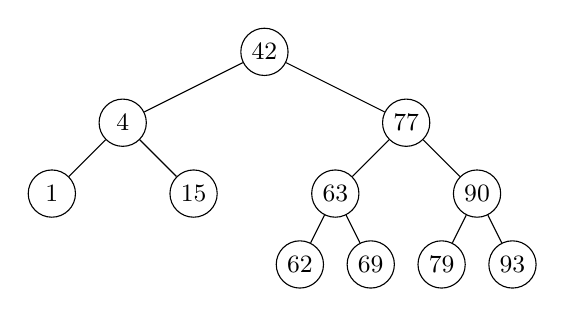
\begin{tikzpicture}[level distance=9mm,every node/.style={circle,draw,minimum size=6mm,inner sep=0pt,font=\small},
  level 1/.style={sibling distance=36mm},level 2/.style={sibling distance=18mm},level 3/.style={sibling distance=9mm}]
\node {42} child {node {4} child {node {1}} child {node {15}}}
  child {node {77} child {node {63} child {node {62}} child {node {69}}} child {node {90} child {node {79}} child {node {93}}}};
\end{tikzpicture}
\end{center}
（$90$ 的左子節點 $79$ 還帶著水平連結 $79 \to 86$，圖中省略。） 層級：$42$、$77$ 是第 $3$ 層，$4$、
$63$、$90$ 是第 $2$ 層。 $4$ 和 $42$ 不同層。

\textbf{(D) 插入 61：錯。} 路徑 $77 \to 42 \to 63 \to 62$，$61 < 62$，接在 $62$ 的左邊。 在 $62$：左子節點同層，
skew，$61$ 升上來，$62$ 成為它的右子節點（水平連結）。 split 看 $61 \to 62 \to$（空），不用。 再往上，
$63$ 的左子節點 $61$ 在第 $1$ 層，比 $63$ 低，正常；$42 \to 63 \to 69$ 中 $69$ 在第 $1$ 層，不用 split。
$61$ 的父節點是 $63$，$62$ 反而成了 $61$ 的右子節點。

\textbf{(E) 插入 88：對。} 路徑 $77 \to 90 \to 79 \to 86$，$88 > 86$，接在 $86$ 的右邊（第 $1$ 層）。 往回走：
在 $86$ 沒事；在 $79$，$79 \to 86 \to 88$ 三個同層，split，$86$ 升到第 $2$ 層，左子節點 $79$、右子節點
$88$；在 $90$，左子節點 $86$ 也是第 $2$ 層，skew，$86$ 升上來，$90$ 成為它的右子節點（水平連結），
$88$ 接到 $90$ 的左邊；$86 \to 90 \to 93$ 中 $93$ 在第 $1$ 層，不用 split；在 $77$，右子節點 $86$ 在
第 $2$ 層，沒事。
\begin{center}
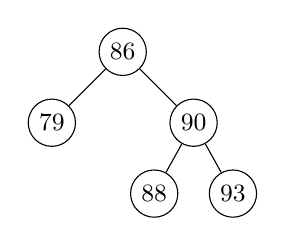
\begin{tikzpicture}[level distance=9mm,every node/.style={circle,draw,minimum size=6mm,inner sep=0pt,font=\small},
  level 1/.style={sibling distance=18mm},level 2/.style={sibling distance=10mm}]
\node {86} child {node {79}} child {node {90} child {node {88}} child {node {93}}};
\end{tikzpicture}
\end{center}
這棵是 $77$ 的右子樹，$86$ 的父節點是 $77$。
\end{pastsoln}
